% -*- coding: utf-8 -*-
\documentclass[UTF8,a4paper,10pt]{ctexart}
\usepackage[left=3.17cm, right=3.17cm, top=2.74cm, bottom=2.74cm]{geometry}
\usepackage{amsmath}
\usepackage{graphicx}
\usepackage{float}
\usepackage{booktabs}
\usepackage{multirow}
\usepackage{caption}
\usepackage{subcaption}
\usepackage{tabularx}
\usepackage{array}
\usepackage{makecell}
\usepackage{enumerate}
\usepackage{enumitem}
\usepackage{xcolor}
\usepackage{listings}
\usepackage[most]{tcolorbox}
\usepackage[colorlinks,linkcolor=black,anchorcolor=blue,hypertexnames=false]{hyperref}
\usepackage{fancyhdr}
\usepackage{tikz}
\usetikzlibrary{fit}
\usepackage{eso-pic}

%-------------------------字体设置--------------
\newcommand{\yihao}{\fontsize{26pt}{36pt}\selectfont}
\newcommand{\erhao}{\fontsize{22pt}{28pt}\selectfont}
\newcommand{\xiaoer}{\fontsize{18pt}{18pt}\selectfont}
\newcommand{\sanhao}{\fontsize{16pt}{24pt}\selectfont}
\newcommand{\xiaosan}{\fontsize{15pt}{22pt}\selectfont}
\newcommand{\sihao}{\fontsize{14pt}{21pt}\selectfont}
\newcommand{\xiaosi}{\fontsize{12pt}{20pt}\selectfont}
\newcommand{\wuhao}{\fontsize{10.5pt}{15.75pt}\selectfont}

%-------------------------章节名----------------
\ctexset{
  section = {
    name = {,、},
    number = \chinese{section}
  },
  subsection = {
    name = {（,）},
    number = \chinese{subsection}
  },
  subsubsection = {
    name = {,},
    number = \arabic{subsubsection}.
  }
}

%-------------------------页眉页脚--------------
\pagestyle{fancy}
\lhead{\kaishu \leftmark}
\rhead{\kaishu PageRank 评分计算实验报告}
\lfoot{}
\cfoot{\thepage}
\rfoot{}
\renewcommand{\headrulewidth}{0.1pt}
\renewcommand{\footrulewidth}{0pt}
\newcommand{\HRule}{\rule{\linewidth}{0.5mm}}
\newcommand{\HRulegrossa}{\rule{\linewidth}{1.2mm}}

%------------------------代码-------------------
\lstset{
breaklines=true,
breakatwhitespace=false,
columns=flexible,
basicstyle=\small\ttfamily,
escapeinside={(*@}{@*)},
keywordstyle=\color[RGB]{0,0,180}\bfseries,
commentstyle=\color[RGB]{106,153,85},
stringstyle=\color[RGB]{163,21,21},
extendedchars=false,
linewidth=\textwidth,
numbers=left,
numberstyle=\tiny \color{blue!50},
frame=trbl,
rulesepcolor=\color{red!20!green!20!blue!20},
captionpos=b
}
\DeclareCaptionFormat{lstnocounter}{\small\textbf{代码\thelstlisting：#3}}
\captionsetup[lstlisting]{format=lstnocounter, singlelinecheck=true, skip=2pt, justification=centering}
\setlength{\emergencystretch}{3em}
\hbadness=2000
\newcolumntype{Y}{>{\raggedright\arraybackslash}X}

%------------------------水印-------------------
\newcommand{\watermark}[3]{\AddToShipoutPictureBG{
\parbox[b][\paperheight]{\paperwidth}{
\vfill
\centering
\tikz[remember picture, overlay]
  \node [rotate = #1, scale = #2] at (current page.center)
    {\textcolor{gray!80!cyan!30!magenta!30}{#3}};
\vfill}}}

\begin{document}
\begin{titlepage}
  \begin{center}
    
\includegraphics[width=0.68\textwidth]{NKU.png}\\[0.35cm]
    {\Huge \kaishu 南\ \ \ \ \ \ 开\ \ \ \ \ \ 大\ \ \ \ \ \ 学}\\[0.35cm]
    {\Large \textbf{大数据计算课程第一次作业}}\\[0.35cm]
    \HRule \\[0.35cm]
    { \LARGE \bfseries PageRank 评分计算实验报告}\\[0.3cm]
    \HRule \\[0.65cm]
    {\small \kaishu
    \renewcommand{\arraystretch}{1.22}
    \begin{tabularx}{0.96\textwidth}{>{\centering\arraybackslash}X|>{\centering\arraybackslash}X|>{\centering\arraybackslash}X}
      \textbf{成员一} & \textbf{成员二} & \textbf{成员三} \\
      \hline
      密码与网络空间安全学院 & 计算机学院 & 计算机学院 \\
      2023级 & 2023级 & 2023级 \\
      信息安全班 & 计算机科学卓越班 & 计算机科学卓越班 \\
      2311208 & 2310428 & 2311671 \\
      魏来 & 韩琦卓 & 侯嘉栋 \\
    \end{tabularx}}\\[0.35cm]
    \vfill
    {\Large \today}
  \end{center}
\end{titlepage}

\tableofcontents
\newpage
\watermark{60}{10}{NKU}
\setcounter{page}{1}

\section{实验摘要}
\xiaosi

\begin{tcolorbox}[colback=blue!3!white,colframe=blue!55!black,title=核心结论]
  本实验在 \texttt{Data.txt} 上独立实现 PageRank，默认采用 $\alpha=0.85$。程序使用节点压缩、CSR Sparse Matrix、源节点区间 Block Matrix 遍历、dead-end 质量回补、spider-trap 传送项和 $L_1$ 残差收敛判定。最终 Top-100 写入 \texttt{result/Res.txt}；静态 Linux x86-64 可执行文件 5 次运行平均耗时约 0.167 s，采样峰值 RSS 约 11.23 MB，远低于 60 s 和 80 MB 限制。
\end{tcolorbox}

\begin{table}[H]
  \centering
  \caption{实验关键指标一览}
  \begin{tabular}{c c c c c c}
    \toprule
    \textbf{节点} & \textbf{边} & \textbf{dead-end} & \textbf{收敛轮数} & \textbf{最终残差} & \textbf{Top1 节点} \\
    \midrule
    9500 & 150000 & 1000 & 17 & $8.064961\times10^{-13}$ & 75 \\
    \bottomrule
  \end{tabular}
\end{table}

\section{实验目的}
\xiaosi

PageRank 是图数据分析中最经典的节点重要性排序算法之一。它把网页、论文、社交账号等对象抽象为有向图中的节点，把引用、链接或关注关系抽象为有向边，并通过带随机跳转的随机游走过程衡量节点的重要程度。本次实验围绕课程给定的 \texttt{Data.txt} 数据集，独立实现 PageRank 评分计算程序，主要目标如下：

\begin{enumerate}
  \item 理解 PageRank 的随机游走模型，掌握阻尼系数、随机跳转、死端节点和蜘蛛陷阱的数学处理方法。
  \item 使用 C++17 从零实现 PageRank，不调用现成 PageRank API，能够读取边列表数据并输出分数最高的前 100 个节点。
  \item 针对稀疏有向图设计紧凑的数据结构，通过节点编号压缩、CSR 稀疏存储和分块迭代降低内存占用。
  \item 使用严格的收敛判定保证结果稳定，并通过编译运行、输出检查和性能统计验证程序满足实验限制。
\end{enumerate}

\section{实验内容}
\xiaosi

本实验完成的核心工作包括：

\begin{enumerate}
  \item 对 \texttt{Data.txt} 进行两遍扫描：第一遍收集所有实际出现的节点并统计边数，第二遍将原始边压缩为连续下标边。
  \item 对原始节点编号排序去重，建立从原始节点 ID 到连续数组下标的映射，使 PageRank 向量、出度数组和邻接结构只按真实节点数量分配。
  \item 使用 CSR（Compressed Sparse Row）结构保存稀疏有向图，不构造 $N \times N$ 的稠密邻接矩阵。
  \item 以阻尼系数 $\alpha=0.85$ 进行 PageRank 迭代，显式处理 dead-end 节点，并使用随机跳转项消除 spider-trap 的局部吸收。
  \item 在迭代阶段按源节点连续区间进行行块遍历，结合预计算出边权重、归一化和 Top-K 部分排序优化程序性能。
  \item 将最终 PageRank 分数最高的 100 个节点写入 \texttt{result/Res.txt}，并记录运行规模、收敛轮数、残差和内存时间表现。
\end{enumerate}

\section{数据集描述}
\xiaosi

本实验使用作业给定数据集 \texttt{Data.txt}。文件每一行包含两个整数：

\begin{lstlisting}[language=bash, caption={Data.txt 数据格式}]
FromNodeID ToNodeID
\end{lstlisting}

其中 \texttt{FromNodeID} 表示有向边起点，\texttt{ToNodeID} 表示有向边终点，即一条从起点指向终点的链接关系。程序只将文件中实际出现过的节点纳入计算，对原始节点编号进行连续化映射后再执行 PageRank。

本次运行时程序扫描得到的数据规模如下：

\begin{table}[H]
  \centering
  \caption{数据集基础统计信息}
  \begin{tabular}{cc}
    \toprule
    \textbf{项目} & \textbf{统计值} \\
    \midrule
    节点数 & 9500 \\
    有向边数 & 150000 \\
    死端节点数 & 1000 \\
    重复边数 & 0 \\
    节点编号范围 & 0 到 9999 \\
    最大入度 / 最大出度 & 32 / 36 \\
    图密度 $M/N^2$ & 约 0.166\% \\
    迭代块大小 & 1024 个源节点 \\
    \bottomrule
  \end{tabular}
\end{table}

\begin{figure}[H]
  \centering
  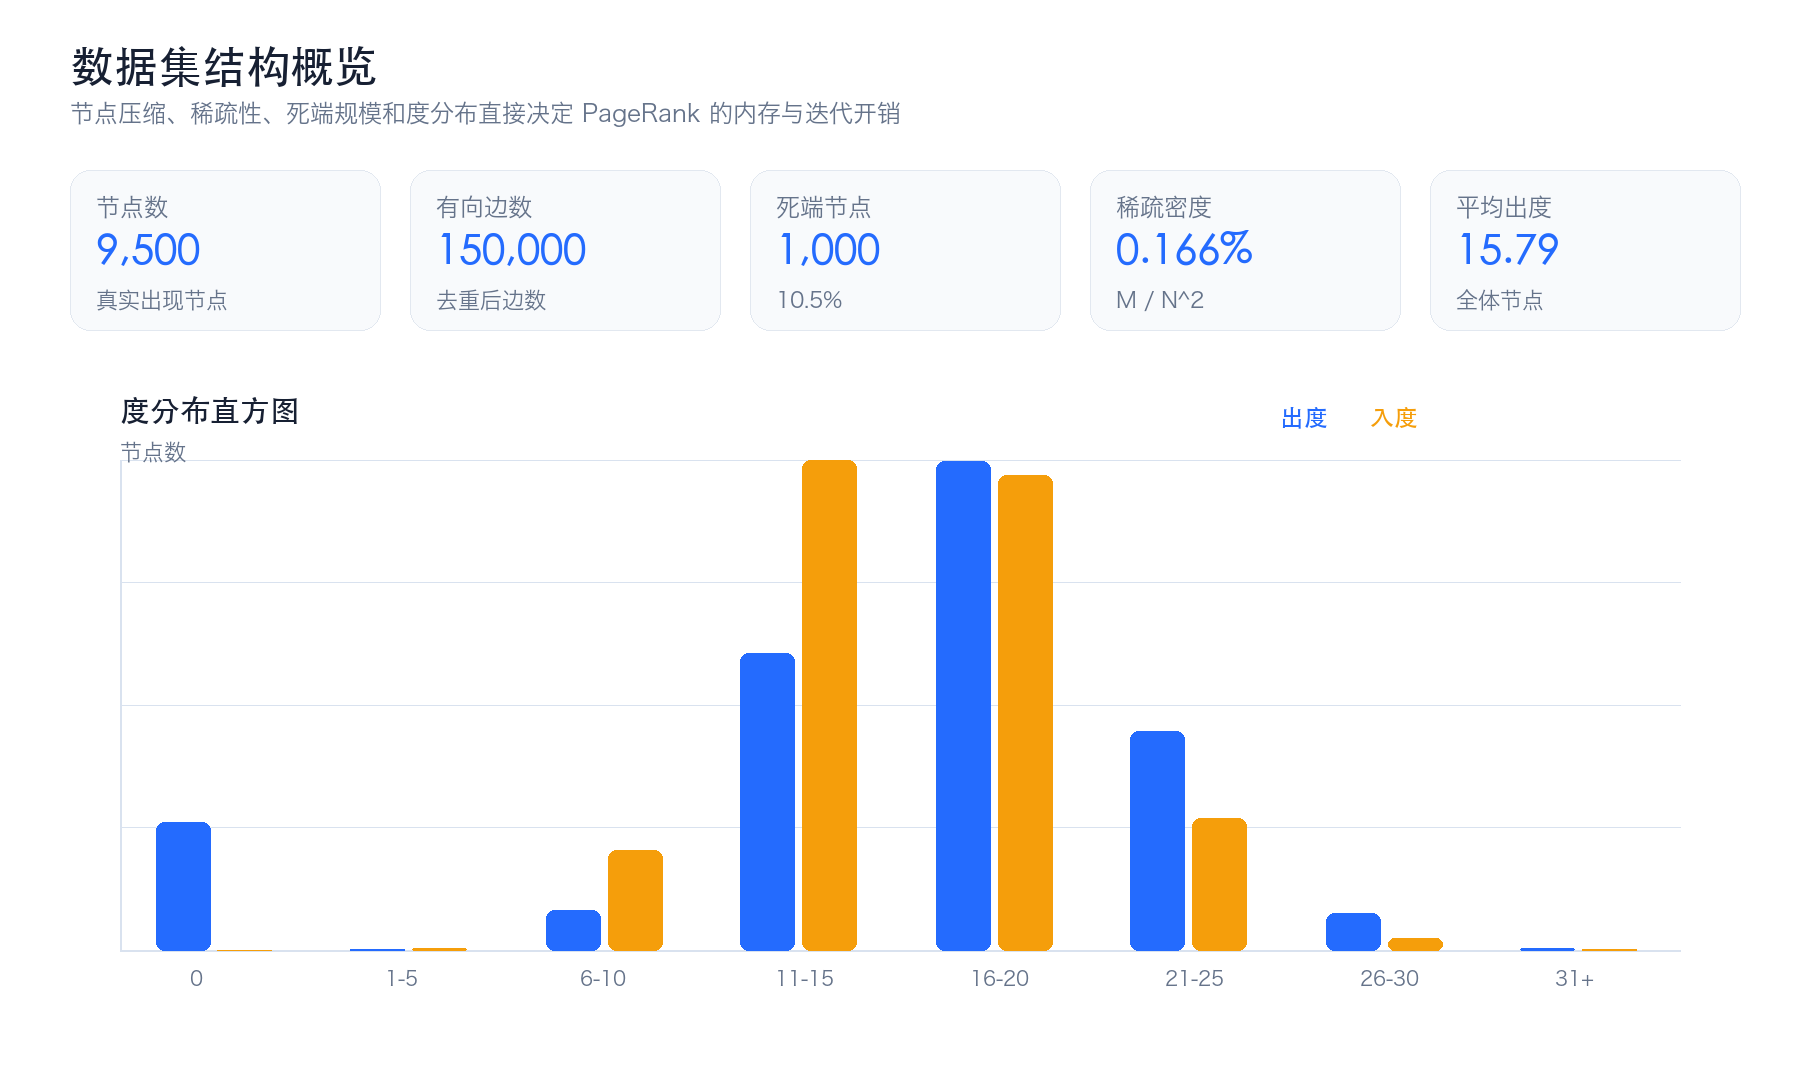
\includegraphics[width=\textwidth]{images/dataset_overview.png}
  \caption{数据集结构、稀疏性与度分布统计}
  \label{fig:dataset-overview}
\end{figure}

\begin{tcolorbox}[colback=cyan!5!white,colframe=cyan!75!black,title=数据集处理说明]
  \hspace{2em}虽然本数据集中节点编号位于 0 到 9999 之间，但实际出现的节点只有 9500 个。如果直接按照最大编号开辟数组，会为未出现的节点分配无意义空间；如果进一步构造稠密矩阵，空间浪费会放大到平方级。因此程序首先收集所有出现过的节点，排序去重后建立连续下标，再在压缩图上执行 PageRank。
\end{tcolorbox}

\section{实验原理}
\xiaosi

\subsection{从链接图到随机游走}

PageRank 将网页链接图抽象为有向图 $G=(V,E)$。节点表示网页或实体，有向边 $u\rightarrow v$ 表示从 $u$ 指向 $v$ 的链接。它可以解释为“随机浏览者”模型：用户当前位于某节点时，要么沿当前节点的一条出边随机前进，要么执行一次全局随机跳转；长期访问频率越高的节点越重要。

设 $N=|V|$，$A$ 为邻接矩阵，若存在边 $u\rightarrow v$ 则 $A_{uv}=1$。若节点 $u$ 出度为 $out(u)>0$，则从 $u$ 沿每条出边转移的概率为：

\begin{equation}
P_{uv}=\frac{A_{uv}}{out(u)}
\end{equation}

矩阵 $P$ 是行随机矩阵，每一行概率和为 1。PageRank 向量可视为马尔可夫链的平稳分布；幂迭代不断计算 $r_{t+1}=r_tP$，直到相邻两轮变化足够小。

\subsection{传送项与 Google 矩阵}

仅沿链接随机游走会遇到两个问题：一是 dead-end 节点没有出边，概率质量无法继续传播；二是 spider-trap 结构会把概率质量困在局部闭环中。PageRank 因此引入传送机制。本实验将作业指定的 teleport parameter 0.85 按 PageRank 常用写法解释为 damping factor $\alpha=0.85$：以 $\alpha$ 的权重沿链接传播，以 $1-\alpha$ 的权重均匀跳转到任意节点。对应 Google 矩阵可写为：

\begin{equation}
G=\alpha P + (1-\alpha)\frac{\mathbf{1}\mathbf{1}^{T}}{N}
\end{equation}

实际实现不显式构造 $G$。原因是传送矩阵为稠密矩阵，若直接保存会破坏稀疏性；程序把传送项合并为每轮统一基值：

\begin{equation}
base=\frac{1-\alpha}{N}
\end{equation}

然后仅沿真实边执行稀疏传播。

\subsection{dead-end 质量回补}

dead-end 节点指 $out(u)=0$ 的节点。若忽略这类节点，其 PageRank 质量不会分配给任何目标节点，向量和会持续下降。设 dead-end 集合为 $D$，第 $t$ 轮 dead-end 总质量为：

\begin{equation}
M_t=\sum_{u\in D}r_t(u)
\end{equation}

随机浏览者到达 dead-end 后应等概率跳转到任意节点，因此每个节点获得的 dead-end 回补为：

\begin{equation}
dead\_share=\alpha\frac{M_t}{N}
\end{equation}

本实验最终采用的更新公式为：

\begin{equation}
r_{t+1}(v)=\frac{1-\alpha}{N}
+\alpha\frac{M_t}{N}
+\alpha\sum_{u\in In(v)}\frac{r_t(u)}{out(u)}
\end{equation}

其中 $In(v)$ 为指向 $v$ 的入邻居集合。该公式同时处理了随机跳转、dead-end 和普通链接传播。

\begin{figure}[H]
  \centering
  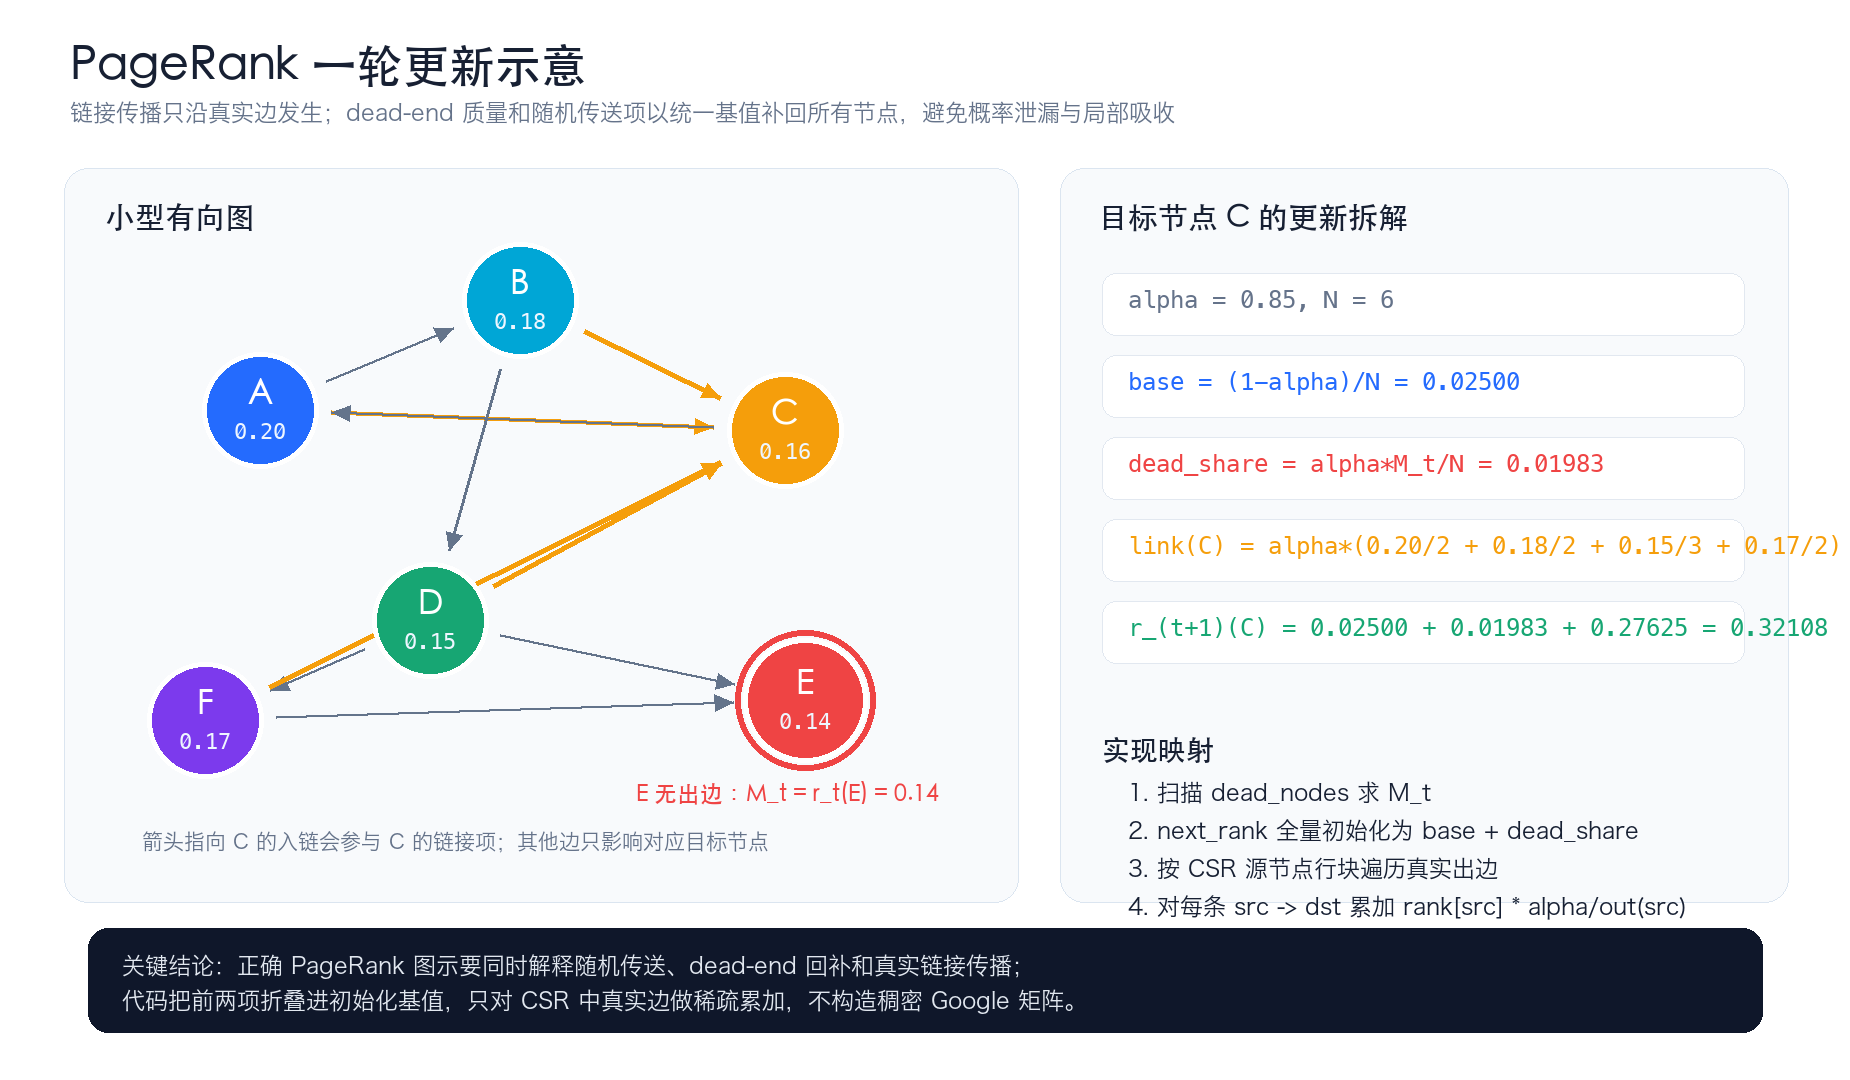
\includegraphics[width=\textwidth]{images/pagerank_principle_example.png}
  \caption{PageRank 一轮更新的质量来源拆解}
  \label{fig:pagerank-principle-example}
\end{figure}

\begin{tcolorbox}[colback=blue!3!white,colframe=blue!55!black,title=原理示例分析]
  \hspace{2em}图~\ref{fig:pagerank-principle-example} 使用 6 个节点的小图展示一次迭代的完整质量闭合。目标节点 $C$ 的下一轮分数由三部分构成：全局随机传送项 $(1-\alpha)/N$、dead-end 节点 $E$ 的质量回补 $\alpha M_t/N$、以及所有入邻居按出度拆分后的链接贡献。该图刻意保留 dead-end 节点，是因为只画普通入链会掩盖 PageRank 实现中最容易出错的概率泄漏问题；当前代码正是先计算 $M_t$，再把 \texttt{next\_rank} 初始化为 \texttt{base + dead\_share}，最后只沿 CSR 中真实边累加链接项。
\end{tcolorbox}

\subsection{spider-trap 的数学含义}

spider-trap 是一组具有内部闭合链接结构的节点。若没有传送项，一旦随机游走进入该集合，概率质量会在集合内部循环，外部节点的 PageRank 被系统性低估。传送项 $(1-\alpha)/N$ 使每个节点每轮都获得正概率，因此马尔可夫链更容易满足不可约和非周期条件，长期分布稳定存在。当前 $\alpha=0.85$ 的含义是：链接结构仍占主导，但每轮保留 15\% 的全局探索能力。

\subsection{幂迭代与收敛判定}

本实验使用幂迭代计算平稳分布。初始化时所有节点等概率：

\begin{equation}
r_0(v)=\frac{1}{N}
\end{equation}

每轮根据上式更新 $r_{t+1}$。为了降低浮点误差累积，程序每轮对 $r_{t+1}$ 做归一化，使 $\sum_v r_{t+1}(v)=1$。收敛指标使用相邻两轮向量的 $L_1$ 残差：

\begin{equation}
diff_t=\sum_{v=1}^{N}|r_{t+1}(v)-r_t(v)|
\end{equation}

当 $diff_t<10^{-12}$ 时停止。$L_1$ 残差直接衡量整个概率分布的总变化量，比只比较单个节点最大误差更适合描述 PageRank 向量的整体稳定性。

\subsection{稀疏矩阵与块矩阵视角}

PageRank 每轮迭代本质上是一次稀疏矩阵向量乘法。若保存稠密矩阵，空间复杂度为 $O(N^2)$；对本数据集 $N=9500$，仅一个 double 矩阵就约需 688.55 MB。课程要求使用 Sparse Matrix 和 Block Matrix，因此程序以 CSR 表示稀疏转移结构，把空间复杂度降为 $O(N+M)$，并按源节点行区间分块扫描 CSR。本实现的 Block Matrix 不是为了改变数学模型，而是为了把每轮传播组织为更稳定的行块工作集：

\begin{equation}
A=
\begin{bmatrix}
A_{0}\\
A_{1}\\
\vdots\\
A_{k}
\end{bmatrix},\qquad
r_{t+1}=\sum_{i=0}^{k}\alpha A_i^{T}r_t + base + dead\_share
\end{equation}

其中 $A_i$ 表示一段连续源节点对应的稀疏行块。这样既满足块矩阵优化要求，也保持实现简单、可验证。

\section{算法设计与内存优化}
\xiaosi

\subsection{总体流程}

当前优化后的程序以 \texttt{Graph} 结构作为核心数据载体，内部包含压缩后的原始节点表 \texttt{node\_ids}、CSR 行指针 \texttt{row\_ptr}、目标节点数组 \texttt{col\_idx}、预计算出边权重 \texttt{out\_weight} 和死端节点列表 \texttt{dead\_nodes}。程序整体流程如图~\ref{fig:pagerank-flow} 所示：先完成节点压缩和稀疏图构建，再在 CSR 结构上执行 PageRank 迭代，最后用部分排序得到 Top-100 结果。

\begin{figure}[H]
  \centering
  \begin{tikzpicture}[>=stealth, thick, font=\small,
    stage/.style={draw=gray!55, rounded corners, inner sep=8pt},
    box/.style={draw, rounded corners=3pt, align=center, minimum width=3.9cm, minimum height=0.82cm},
    prep/.style={box, fill=cyan!7},
    block/.style={box, fill=green!8},
    iter/.style={box, fill=blue!7},
    result/.style={box, fill=orange!10}]

    \node[prep] (a1) at (0,0) {读取 \texttt{Data.txt}};
    \node[prep] (a2) at (0,-1.15) {收集节点并统计边数};
    \node[prep] (a3) at (0,-2.30) {节点排序去重};
    \node[prep] (a4) at (0,-3.45) {建立编号映射};
    \node[stage, fit=(a1)(a2)(a3)(a4), label={[font=\bfseries]above:预处理}] {};

    \node[block] (b1) at (6.0,-0.55) {压缩并打包边};
    \node[block] (b2) at (6.0,-1.70) {边排序去重};
    \node[block] (b3) at (6.0,-2.85) {生成 CSR 稀疏图};
    \node[stage, fit=(b1)(b2)(b3), label={[font=\bfseries]above:图结构构建}] {};

    \node[iter] (c1) at (0,-6.00) {计算死端节点贡献};
    \node[iter] (c2) at (0,-7.15) {初始化下一轮分数};
    \node[iter] (c3) at (0,-8.30) {按源节点块遍历 CSR};
    \node[iter] (c4) at (0,-9.45) {判断 $L_1$ 收敛};
    \node[stage, fit=(c1)(c2)(c3)(c4), label={[font=\bfseries]above:PageRank 迭代}] {};

    \node[result] (d1) at (6.0,-6.55) {部分排序节点索引};
    \node[result] (d2) at (6.0,-7.70) {还原原始节点编号};
    \node[result] (d3) at (6.0,-8.85) {写出 \texttt{Res.txt}};
    \node[stage, fit=(d1)(d2)(d3), label={[font=\bfseries]above:结果输出}] {};

    \draw[->] (a1) -- (a2);
    \draw[->] (a2) -- (a3);
    \draw[->] (a3) -- (a4);
    \draw[->] (a4.east) -- ++(0.7,0) |- (b1.west);
    \draw[->] (b1) -- (b2);
    \draw[->] (b2) -- (b3);
    \draw[->] (b3.south) -- ++(0,-1.15) -| (c1.north);
    \draw[->] (c1) -- (c2);
    \draw[->] (c2) -- (c3);
    \draw[->] (c3) -- (c4);
    \draw[->] (c4.east) -- ++(0.7,0) |- (d1.west);
    \draw[->] (d1) -- (d2);
    \draw[->] (d2) -- (d3);
  \end{tikzpicture}
  \caption{PageRank 程序总体流程}
  \label{fig:pagerank-flow}
\end{figure}

\subsection{节点编号压缩}

输入文件中的节点 ID 是外部编号，不能假设其连续、紧凑或从 0 开始。程序第一遍扫描文件时，把每条边的起点和终点都加入 \texttt{node\_ids}，再排序去重得到真实节点集合。后续所有数组均使用连续编号 $[0,N)$ 访问，输出时再通过 \texttt{node\_ids} 还原原始节点 ID。

\begin{lstlisting}[language=C++, caption={节点收集与排序去重}]
while (input >> from >> to) {
    node_ids.push_back(from);
    node_ids.push_back(to);
    ++count;
}

std::sort(node_ids.begin(), node_ids.end());
node_ids.erase(std::unique(node_ids.begin(), node_ids.end()), node_ids.end());
\end{lstlisting}

为了让第二遍读边时能够快速把原始 ID 转换为连续下标，程序实现了 \texttt{NodeIndexer}。当节点编号范围足够紧凑时，\texttt{NodeIndexer} 建立 dense lookup 数组，查找复杂度为 $O(1)$；当节点编号范围过大或过稀疏时，不建立巨大映射表，而是在有序 \texttt{node\_ids} 上使用二分查找，查找复杂度为 $O(\log N)$。这个设计兼顾了当前数据集上的速度和更一般数据集上的内存可控性。

\begin{lstlisting}[language=C++, caption={NodeIndexer 的 dense lookup 判断}]
const std::uint64_t range =
    static_cast<std::uint64_t>(max_id) -
    static_cast<std::uint64_t>(min_id_) + 1;
const std::uint64_t density_limit = node_ids_.size() * 4ull;
if (range > kMaxDenseIdRange || range > density_limit) {
    return;
}
\end{lstlisting}

\subsection{稀疏矩阵优化}

若直接构造 $N\times N$ 邻接矩阵，即使大部分节点之间没有边，也需要为所有位置分配空间。本实验中 $N=9500$，稠密矩阵共有 $9500^2=90250000$ 个位置；如果用 \texttt{double} 保存矩阵元素，仅矩阵本体就需要约 $688.55$ MB，已经远超 80 MB 限制。当前程序没有保存稠密矩阵，而是只保存真实存在的边。

第二遍读入边时，程序先把每条边压缩为连续下标，再打包到一个 64 位整数中。高 32 位保存起点下标，低 32 位保存终点下标。打包后的边可以直接排序和去重，避免使用 \texttt{pair<int,int>} 带来的对象比较和额外结构开销。

\begin{lstlisting}[language=C++, caption={压缩边的 64 位打包}]
PackedEdge PackEdge(int from, int to) {
    return (static_cast<PackedEdge>(static_cast<std::uint32_t>(from)) << 32) |
           static_cast<std::uint32_t>(to);
}
\end{lstlisting}

排序去重后的边表进一步转换为 CSR 结构。CSR 使用 \texttt{row\_ptr} 保存每个源节点出边区间的起止位置，使用 \texttt{col\_idx} 连续保存目标节点。对于节点 \texttt{src}，其出边对应区间为：

\begin{equation}
[\texttt{row\_ptr[src]},\texttt{row\_ptr[src+1]})
\end{equation}

\begin{lstlisting}[language=C++, caption={由压缩边生成 CSR}]
graph.row_ptr.assign(n + 1, 0);
for (const auto& edge : edges) {
    ++graph.row_ptr[EdgeFrom(edge) + 1];
}

for (int i = 0; i < n; ++i) {
    graph.row_ptr[i + 1] += graph.row_ptr[i];
}

graph.col_idx.assign(edges.size(), 0);
for (std::size_t i = 0; i < edges.size(); ++i) {
    graph.col_idx[i] = EdgeTo(edges[i]);
}
\end{lstlisting}

\begin{tcolorbox}[colback=green!5!white,colframe=green!50!black,title=稀疏存储分析]
  \hspace{2em}CSR 的空间复杂度为 $O(N+M)$，其中 $N$ 为节点数，$M$ 为去重后的边数。当前数据集中 $N=9500$、$M=150000$，图结构主要由 9501 个行指针和 150000 个目标节点下标组成，空间规模与真实边数线性相关，避免了稠密矩阵的平方级内存开销。
\end{tcolorbox}

\subsection{块矩阵优化}

PageRank 迭代本质上是稀疏转移矩阵与 PageRank 向量的反复乘法。当前实现没有显式构造矩阵，而是把 CSR 的源节点行按连续区间分块遍历，默认块大小为 1024。对当前 9500 个节点而言，源节点区间可划分为：

\begin{equation}
[0,1024), [1024,2048), \ldots, [9216,9500)
\end{equation}

每一轮迭代中，程序先初始化 \texttt{next\_rank}，再按块处理源节点的所有出边。块内每个源节点的 PageRank 分数乘以预计算的 \texttt{out\_weight[src]} 后，累加到对应目标节点。

\begin{lstlisting}[language=C++, caption={按源节点块遍历 CSR}]
for (int block_start = 0; block_start < n; block_start += kBlockSize) {
    const int block_end = std::min(block_start + kBlockSize, n);
    for (int src = block_start; src < block_end; ++src) {
        const int begin = graph.row_ptr[src];
        const int end = graph.row_ptr[src + 1];
        if (begin == end) {
            continue;
        }

        const double contribution = rank[src] * graph.out_weight[src];
        for (int edge = begin; edge < end; ++edge) {
            next_rank[graph.col_idx[edge]] += contribution;
        }
    }
}
\end{lstlisting}

这种分块方式等价于把稀疏矩阵按行切分为若干块，逐块完成矩阵向量乘法。由于 CSR 中同一源节点的出边连续存储，块内访问 \texttt{row\_ptr} 和 \texttt{col\_idx} 具有较好的顺序性；同时每个块只处理一段源节点，方便控制循环工作集大小，使缓存访问更加稳定。

\begin{figure}[H]
  \centering
  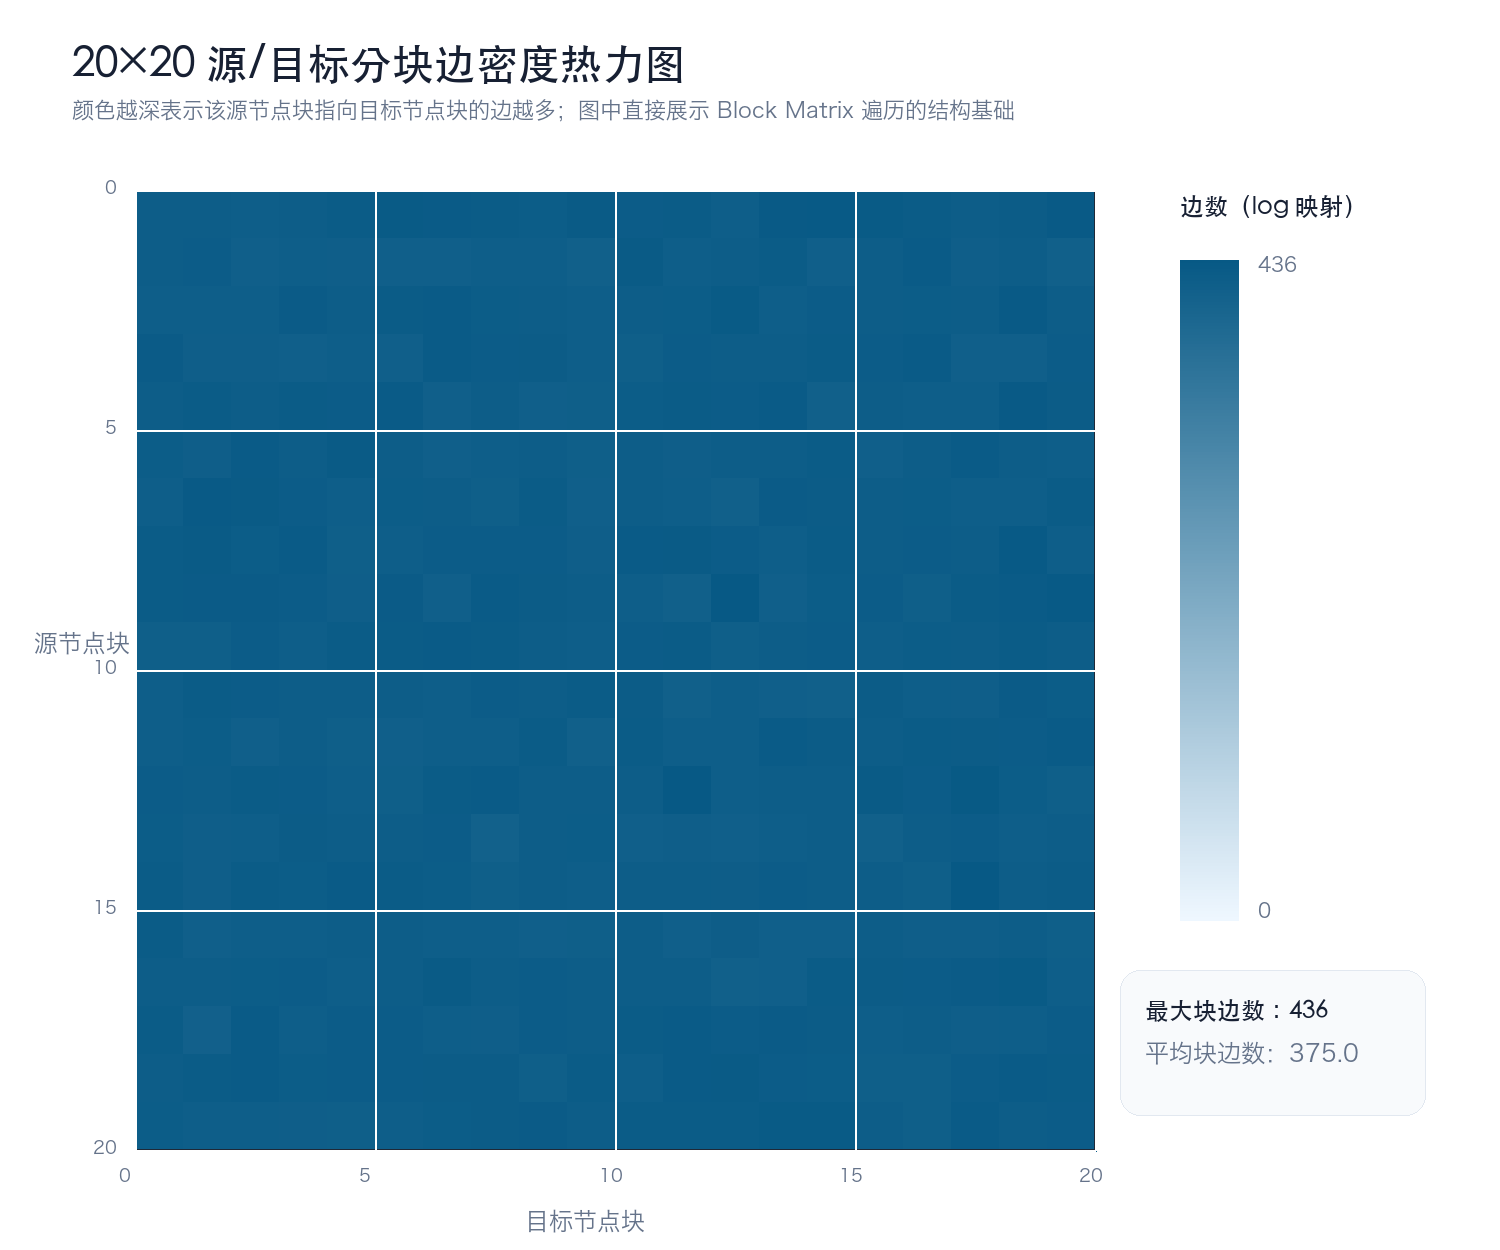
\includegraphics[width=0.88\textwidth]{images/block_heatmap.png}
  \caption{源节点块与目标节点块之间的边密度热力图}
  \label{fig:block-heatmap}
\end{figure}

\begin{tcolorbox}[colback=blue!3!white,colframe=blue!55!black,title=块矩阵分析]
  \hspace{2em}图~\ref{fig:block-heatmap} 将 9500 个压缩节点均匀切成 20 个源块和 20 个目标块。每个格子的颜色表示该源块指向该目标块的边数。虽然本数据集并非网页 URL 排序产生的强对角块结构，但所有格子的边数都在数百量级，说明按源块扫描时每个工作块规模稳定，适合用 CSR 连续区间完成稀疏矩阵向量乘法。
\end{tcolorbox}

\subsection{其他内存与计算优化}

除节点压缩、CSR 稀疏存储和块遍历外，程序还做了以下优化：

\begin{enumerate}
  \item \textbf{两遍读图：} 第一遍只收集节点和边数，第二遍再生成压缩边，避免在读图阶段长期保存原始字符串或复杂边对象。
  \item \textbf{打包边排序：} 使用 64 位整数表示压缩边，使排序去重可以直接比较整数，去除重复边并降低比较开销。
  \item \textbf{出边权重预计算：} 对非死端节点预先保存 $\alpha/out(u)$，迭代时只需要乘法，不再重复执行除法。
  \item \textbf{死端节点单独保存：} 只遍历 \texttt{dead\_nodes} 计算死端质量，不需要每轮扫描全部节点判断出度是否为 0。
  \item \textbf{归一化与残差合并：} 对 \texttt{next\_rank} 归一化的同时计算 $L_1$ 差值，减少一次完整向量遍历。
  \item \textbf{Top-K 部分排序：} 输出阶段使用 \texttt{partial\_sort} 获取前 100 个节点，避免对全部节点进行完整排序。
\end{enumerate}

\subsection{代码结构详细分析}

当前 \texttt{PageRank.cpp} 虽然是单文件提交，但内部按功能边界划分清晰，主要由以下模块组成：

\begin{enumerate}
  \item \textbf{常量与数据结构：} 文件开头集中定义阻尼系数、收敛阈值、最大迭代轮数、输出规模和块大小等算法参数。核心结构 \texttt{Graph} 保存压缩节点表、CSR 图结构、出边权重和死端节点列表，是后续计算的唯一图数据入口。
  \item \textbf{节点映射模块：} \texttt{NodeIndexer} 负责将原始节点 ID 映射到连续下标。它优先使用 dense lookup 数组获得 $O(1)$ 查找；当节点编号范围不适合建立 dense 数组时，退化为二分查找。这一设计避免了 \texttt{unordered\_map} 的哈希桶开销，也不会在稀疏大编号数据上盲目分配巨大数组。
  \item \textbf{读图与压缩模块：} \texttt{ReadNodeIds} 第一遍扫描输入，收集所有端点并排序去重；\texttt{ReadCompressedEdges} 第二遍扫描输入，借助 \texttt{NodeIndexer} 生成压缩边，并通过 \texttt{PackEdge} 打包成 64 位整数。排序去重后再进入 CSR 构建，保证重复边不会污染出度统计。
  \item \textbf{CSR 构建模块：} \texttt{ReadGraph} 先统计每个源节点出边数量，再对 \texttt{row\_ptr} 做前缀和，最后顺序写入 \texttt{col\_idx}。同时，它根据出度判断 dead-end 节点，并为非死端节点预计算 \texttt{out\_weight}。
  \item \textbf{PageRank 迭代模块：} \texttt{ComputePageRank} 是算法核心。每轮先累加死端节点质量，再初始化下一轮向量，然后按源节点块扫描 CSR 出边。迭代尾部对向量归一化并同步计算 $L_1$ 残差，残差低于 $10^{-12}$ 后停止。
  \item \textbf{输出模块：} \texttt{WriteTopRanks} 使用索引数组保存排序对象，通过 \texttt{partial\_sort} 找出前 100 个节点。比较函数先按 PageRank 降序排序，分数相同时按原始节点 ID 升序排序，保证输出稳定。
\end{enumerate}

\begin{table}[H]
  \centering
  \caption{核心函数职责、输入输出与复杂度}
  \small
  \begin{tabularx}{\textwidth}{p{2.8cm} Y Y p{2.4cm}}
    \toprule
    \textbf{函数 / 结构} & \textbf{职责} & \textbf{关键数据} & \textbf{复杂度} \\
    \midrule
    \texttt{ReadNodeIds} & 第一遍扫描输入，收集所有端点并统计原始边数 & \texttt{node\_ids}, \texttt{edge\_count} & $O(M\log M)$ 排序 \\
    \texttt{NodeIndexer} & 原始 ID 到连续下标映射；紧凑 ID 用 dense lookup，稀疏 ID 用二分 & \texttt{dense\_index\_}, \texttt{node\_ids\_} & $O(1)$ 或 $O(\log N)$ \\
    \makecell[l]{\texttt{ReadCompressed}\\\texttt{Edges}} & 第二遍读边、压缩端点、64 位打包、排序去重 & \texttt{PackedEdge} & $O(M\log M)$ \\
    \texttt{ReadGraph} & 基于去重边构建 CSR，并预计算 dead-end 与出边权重 & \texttt{row\_ptr}, \texttt{col\_idx} & $O(N+M)$ \\
    \texttt{ComputePageRank} & 幂迭代、dead-end 回补、分块传播、归一化和残差判断 & \texttt{rank}, \texttt{next\_rank} & $O(T(N+M))$ \\
    \texttt{WriteTopRanks} & 按分数取 Top-100 并恢复原始节点编号 & \texttt{order}, \texttt{node\_ids} & $O(N\log 100)$ \\
    \bottomrule
  \end{tabularx}
\end{table}

从工程角度看，程序的关键不在于堆叠复杂技巧，而是保证每个阶段的数据表示都服务于后续计算：节点压缩使数组紧凑，打包边使去重高效，CSR 使迭代线性扫描真实边，出边权重预计算减少迭代中的重复除法，最后用部分排序避免无意义的全量排序。这些优化共同把 PageRank 的核心开销压缩到真实节点和真实边上。

\section{实验步骤及实验结果}
\xiaosi

\subsection{编译与运行命令}

按照作业要求，C++ 程序使用静态链接方式编译。编译参数文件内容如下：

\begin{lstlisting}[language=bash, caption={compile-parameter.txt}]
g++ -O2 -std=c++17 -static PageRank.cpp -o PageRank.exe
\end{lstlisting}

在仓库根目录下执行：

\begin{lstlisting}[language=bash, caption={编译命令}]
g++ -O2 -std=c++17 -static lab1/src/PageRank.cpp -o lab1/bin/PageRank.exe
\end{lstlisting}

运行：

\begin{lstlisting}[language=bash, caption={运行命令}]
lab1/bin/PageRank.exe lab1/Data.txt lab1/result/Res.txt
\end{lstlisting}

程序运行输出如下：

\begin{lstlisting}[language=bash, caption={程序运行结果}]
nodes: 9500, edges: 150000, iterations: 17, residual: 8.064961e-13
\end{lstlisting}

\begin{figure}[H]
  \centering
  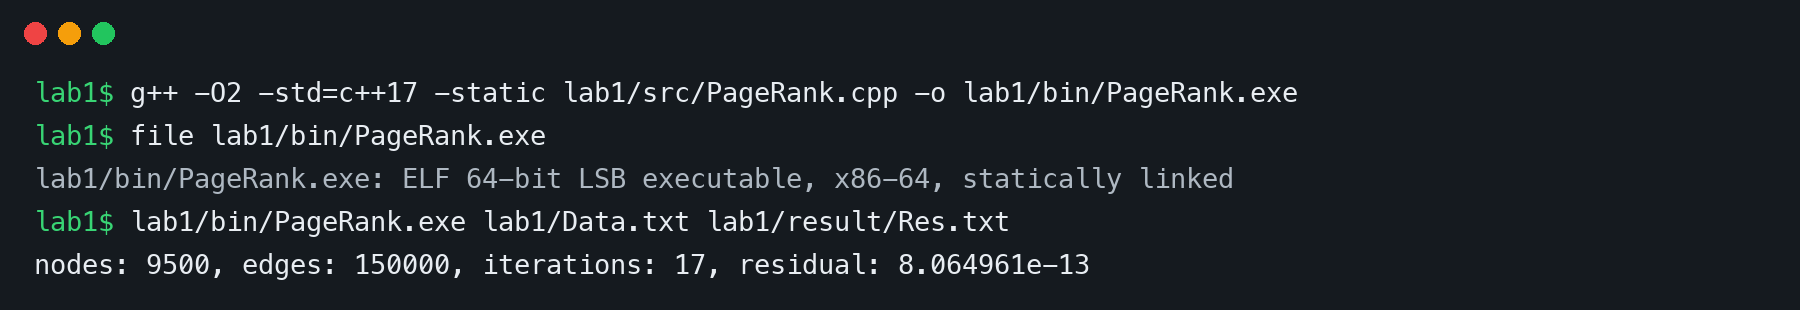
\includegraphics[width=\textwidth]{images/compile_run.png}
  \caption{静态编译、可执行文件检查与运行截图}
  \label{fig:compile-run}
\end{figure}

\subsection{Top-100 输出结果}

输出文件 \texttt{Res.txt} 每行格式为：

\begin{lstlisting}[language=bash, caption={Res.txt 输出格式}]
NodeID Score
\end{lstlisting}

本次实验 Top-20 结果如下，完整 Top-100 已写入 \texttt{Res.txt}：

\begin{table}[H]
  \centering
  \caption{PageRank Top-20 结果（$\alpha=0.85$）}
  \begin{tabular}{ccc}
    \toprule
    \textbf{排名} & \textbf{节点 ID} & \textbf{PageRank 分数} \\
    \midrule
    1 & 75   & 0.000198721357091 \\
    2 & 8686 & 0.000190205478321 \\
    3 & 9678 & 0.000188337048374 \\
    4 & 5104 & 0.00018779534425 \\
    5 & 725  & 0.000186793163631 \\
    6 & 3257 & 0.000185721642407 \\
    7 & 468  & 0.000184900195771 \\
    8 & 7730 & 0.000183938392007 \\
    9 & 7175 & 0.000183838928246 \\
    10 & 5526 & 0.000182843425465 \\
    11 & 8880 & 0.000182589240759 \\
    12 & 6165 & 0.000181381637798 \\
    13 & 2524 & 0.000179768112318 \\
    14 & 7531 & 0.000177955207003 \\
    15 & 9705 & 0.000177273571955 \\
    16 & 6674 & 0.000176715430527 \\
    17 & 5479 & 0.000176315287285 \\
    18 & 8730 & 0.000175446926195 \\
    19 & 5486 & 0.000174638000147 \\
    20 & 579  & 0.000174636519996 \\
    \bottomrule
  \end{tabular}
\end{table}

\begin{figure}[H]
  \centering
  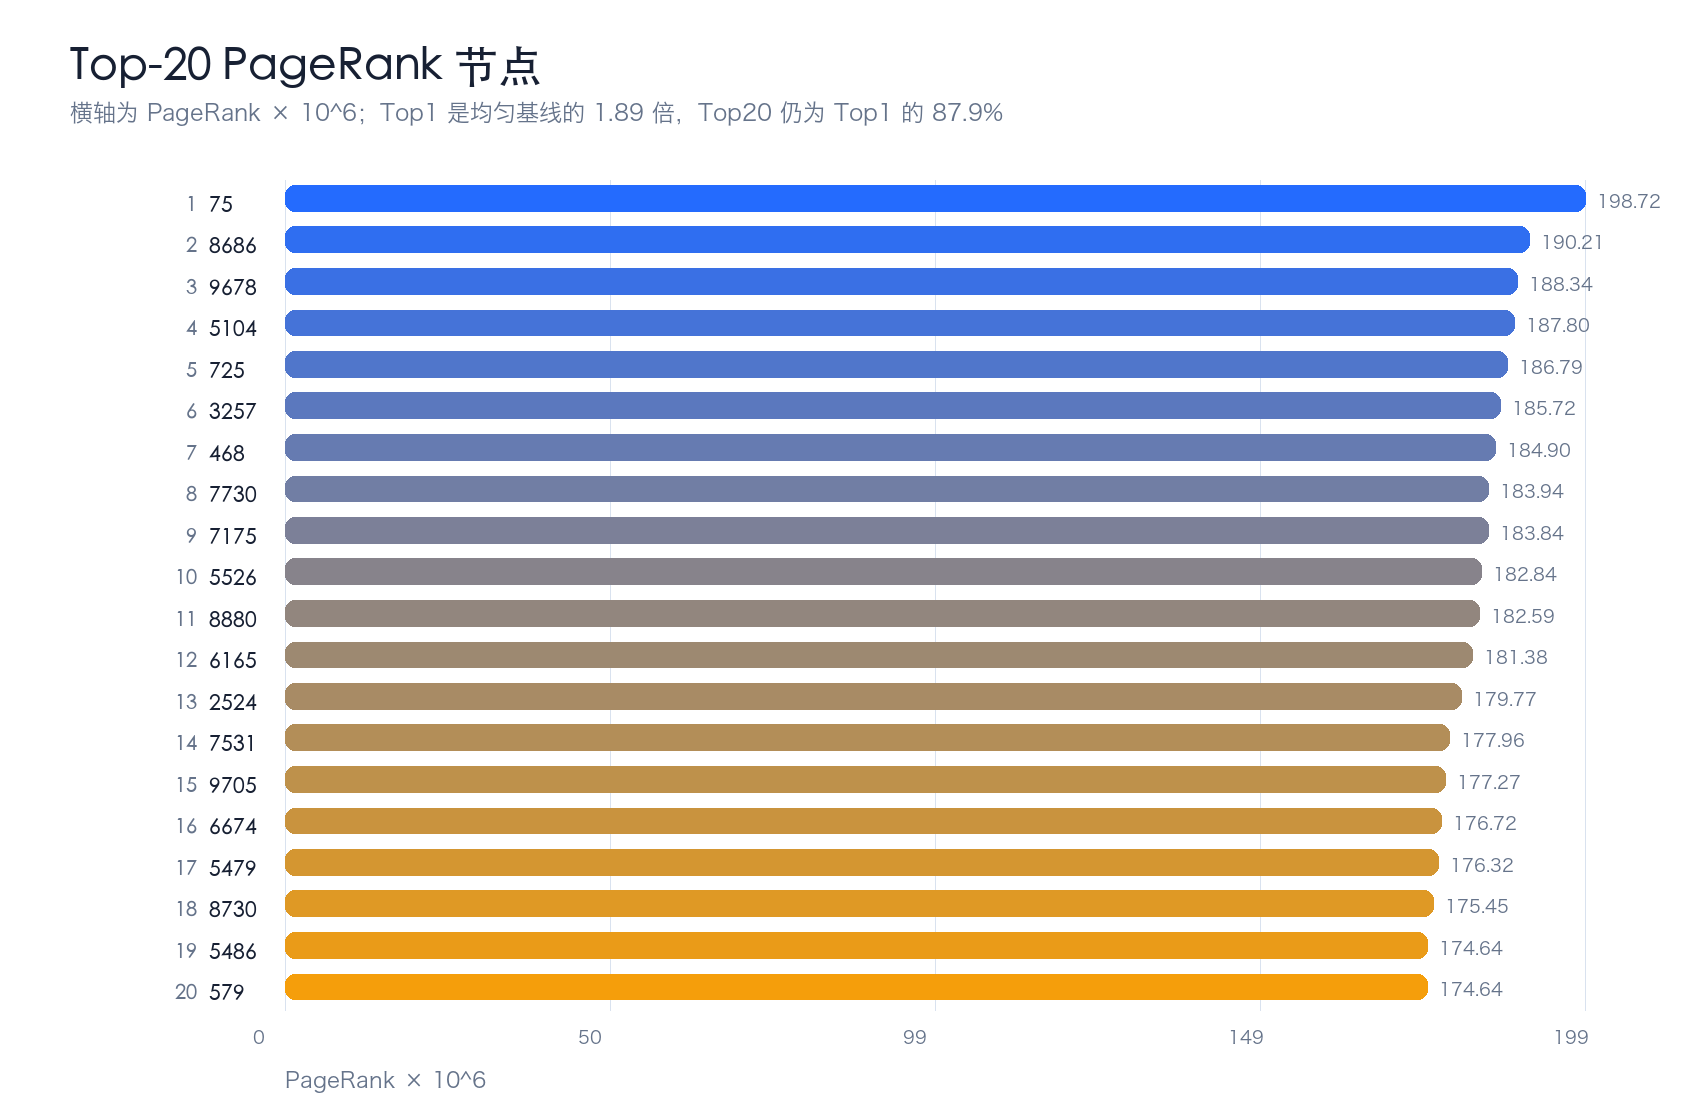
\includegraphics[width=\textwidth]{images/top20_pagerank.png}
  \caption{PageRank Top-20 节点得分可视化}
  \label{fig:top20-pagerank}
\end{figure}

\begin{figure}[H]
  \centering
  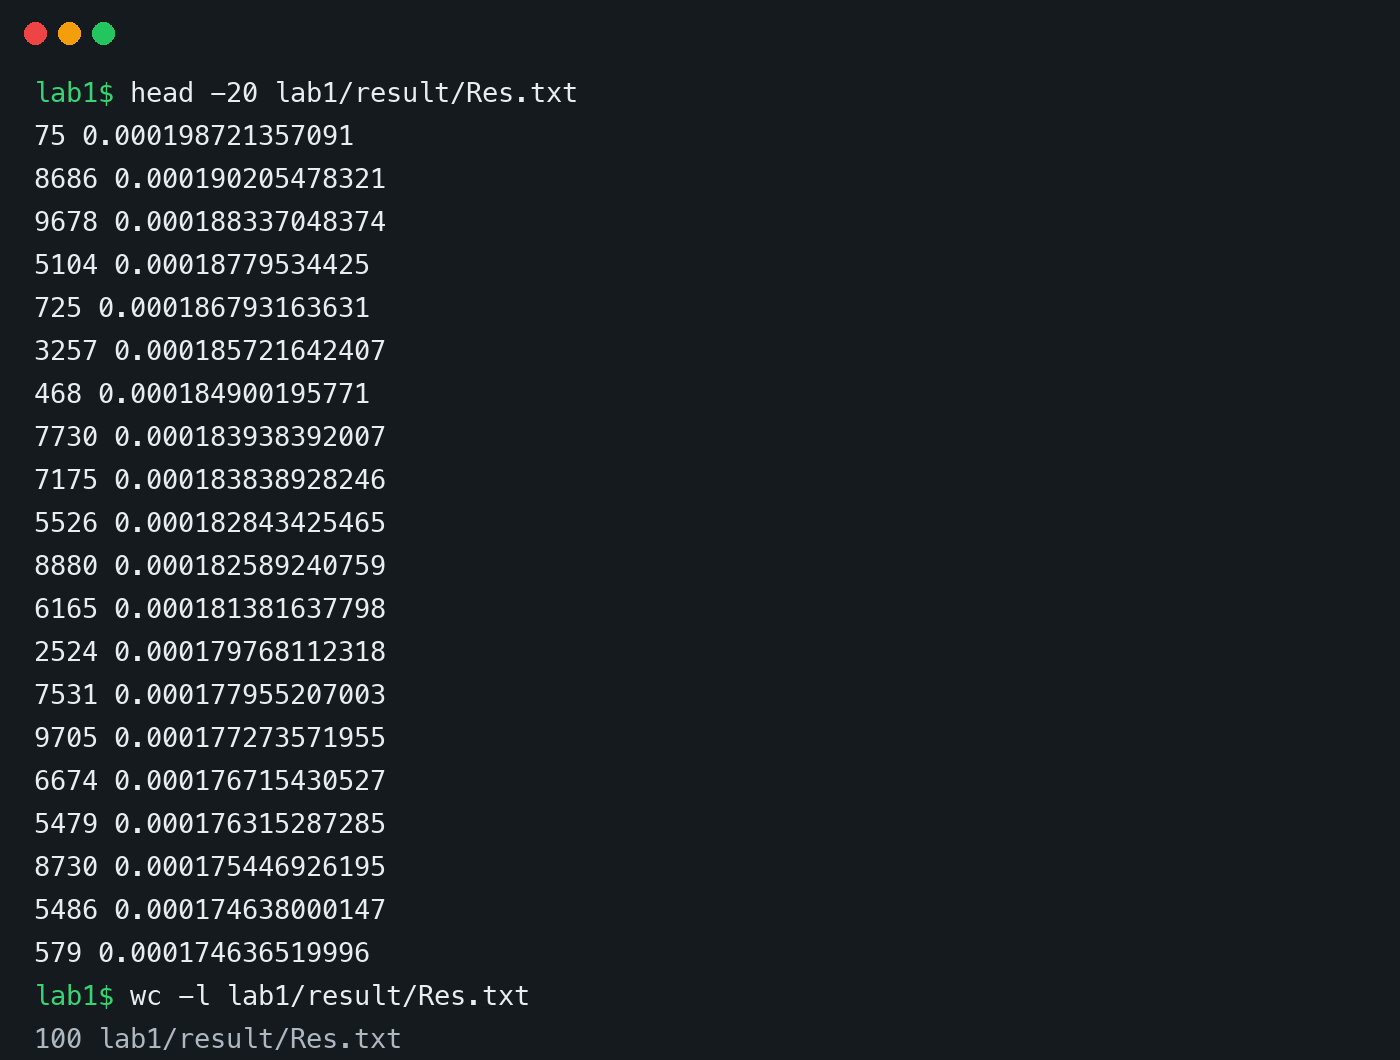
\includegraphics[width=0.82\textwidth]{images/res_output.png}
  \caption{\texttt{Res.txt} 前20行及行数检查}
  \label{fig:res-output}
\end{figure}

\subsection{性能测试命令}

提交文件要求静态链接，因此性能复核以 Linux x86-64 静态可执行文件为准。为同时记录耗时和峰值驻留内存，使用容器内 Python 监控 \texttt{/proc/<pid>/status} 中的 \texttt{VmRSS}，并对同一静态二进制连续运行 5 次：

\begin{lstlisting}[language=bash, caption={单次性能测试命令}]
lab1/bin/PageRank.exe lab1/Data.txt /tmp/Res_static.txt
\end{lstlisting}

\begin{lstlisting}[language=bash, caption={5 次静态可执行文件复核结果}]
1 0.173836 s 11500 KB nodes: 9500, edges: 150000, iterations: 17, residual: 8.064961e-13
2 0.169439 s 11500 KB nodes: 9500, edges: 150000, iterations: 17, residual: 8.064961e-13
3 0.166819 s 11500 KB nodes: 9500, edges: 150000, iterations: 17, residual: 8.064961e-13
4 0.162650 s 11500 KB nodes: 9500, edges: 150000, iterations: 17, residual: 8.064961e-13
5 0.161350 s 11500 KB nodes: 9500, edges: 150000, iterations: 17, residual: 8.064961e-13
\end{lstlisting}

\subsection{性能测试结果}

当前优化版程序 5 次运行均为 17 轮收敛，最终残差约为 $8.064961\times 10^{-13}$。静态 Linux x86-64 二进制平均耗时约 0.167 秒，采样峰值 RSS 约 11.23 MB，远低于 80 MB 内存限制和 60 秒时间限制。

\begin{table}[H]
  \centering
  \caption{当前优化实现性能统计}
  \begin{tabular}{cccccc}
    \toprule
    \textbf{运行次数} & \textbf{迭代次数} & \textbf{最终残差} & \textbf{平均峰值 RSS} & \textbf{平均耗时} & \textbf{最快单次} \\
    \midrule
    5 & 17 & $8.064961\times10^{-13}$ & 约 11.23 MB & 约 0.167 s & 约 0.161 s \\
    \bottomrule
  \end{tabular}
\end{table}

\begin{figure}[H]
  \centering
  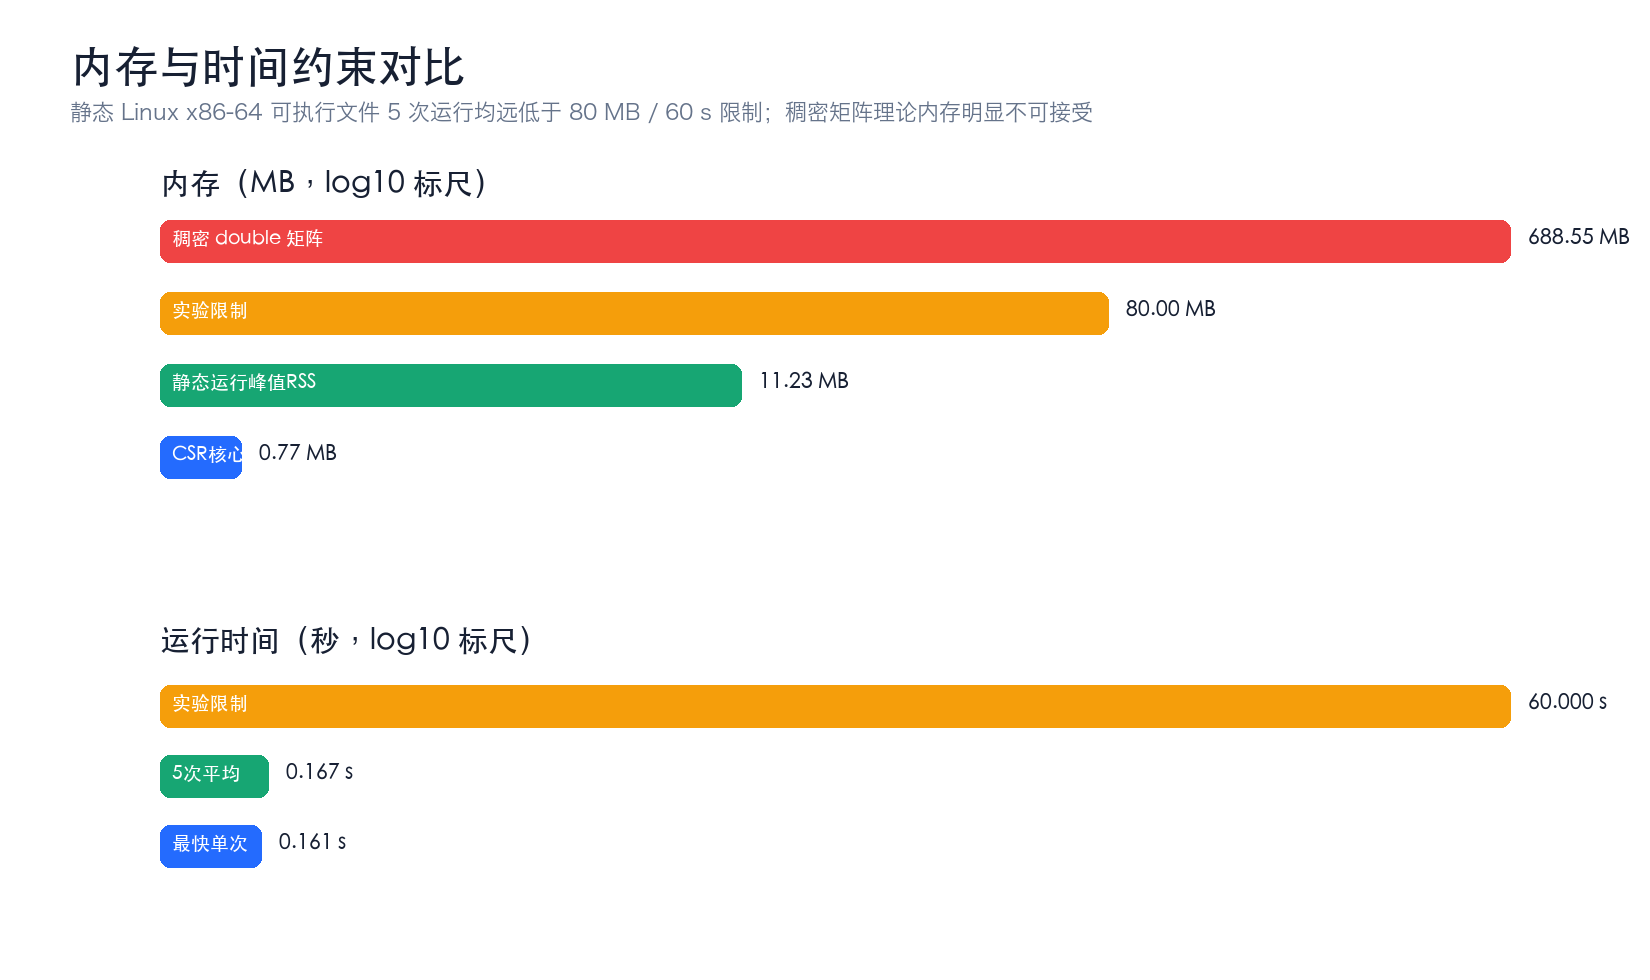
\includegraphics[width=\textwidth]{images/memory_runtime.png}
  \caption{内存与运行时间相对实验限制的对比}
  \label{fig:memory-runtime}
\end{figure}

\subsection{收敛与排名分析}

从收敛曲线看，残差在对数尺度上近似线性下降，说明幂迭代在该图上稳定收敛。dead-end 质量在前几轮迅速稳定，随后每轮被平均回补到全部节点，因此不会发生概率质量泄漏。最终 Top-100 的 PageRank 总和约为 0.01681，Top-20 总和约为 0.00365；Top1 节点 75 的分数约为均匀分布 $1/N$ 的 1.89 倍。

\begin{figure}[H]
  \centering
  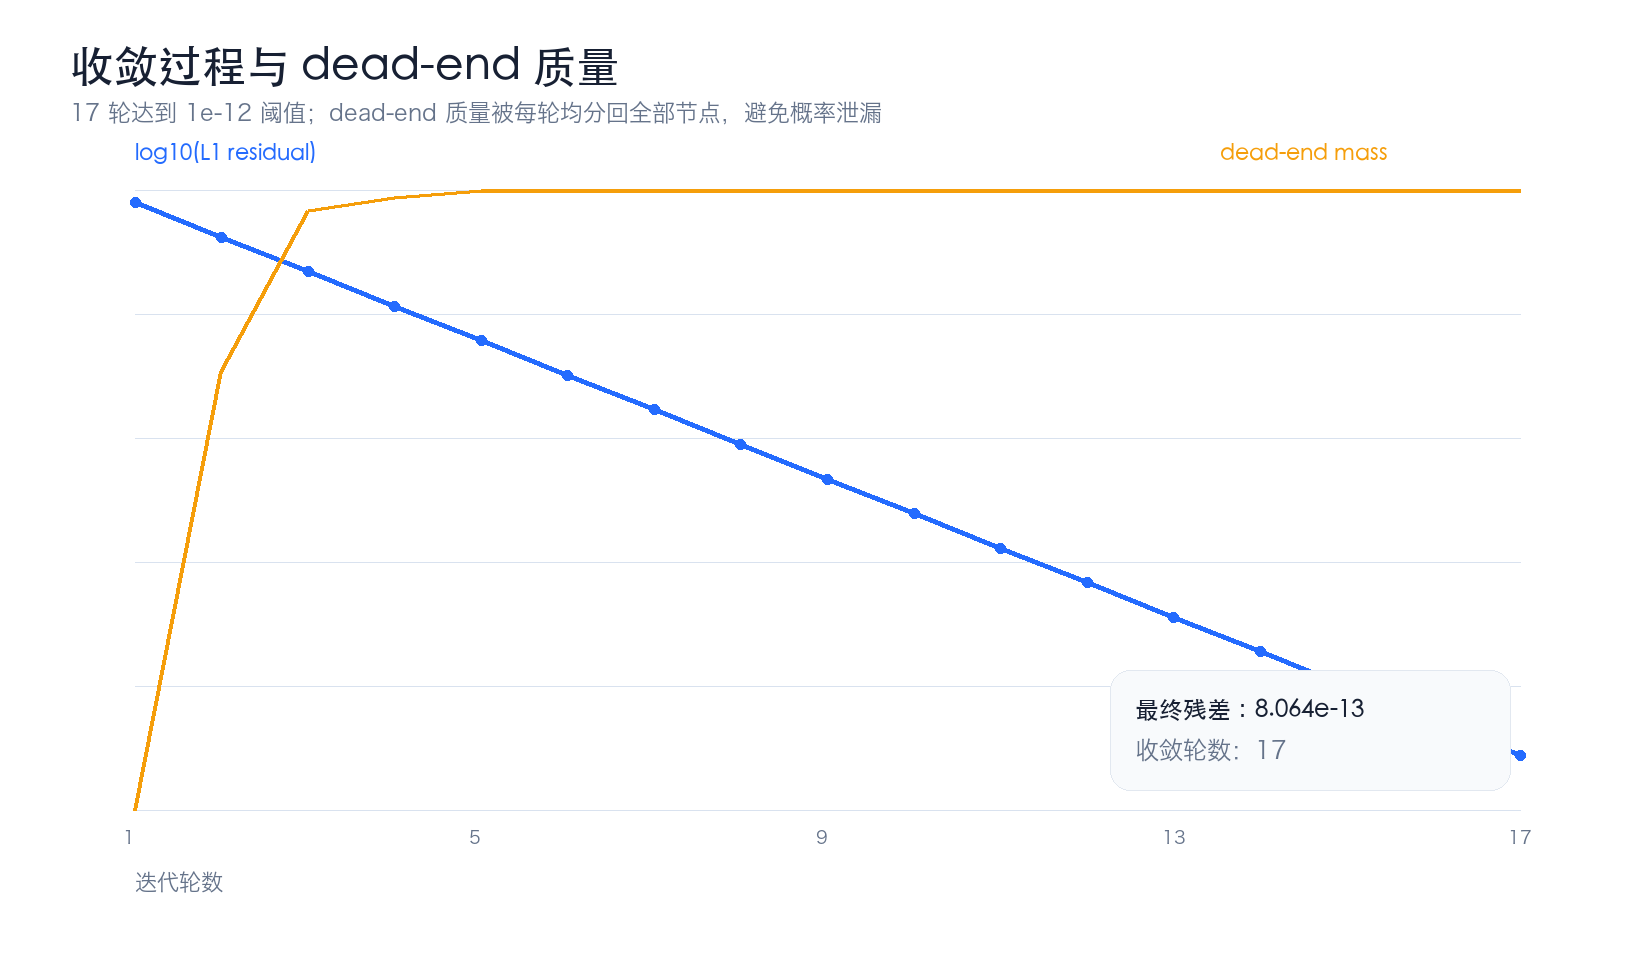
\includegraphics[width=\textwidth]{images/convergence_deadmass.png}
  \caption{PageRank 残差收敛曲线与 dead-end 质量变化}
  \label{fig:convergence-deadmass}
\end{figure}

\begin{figure}[H]
  \centering
  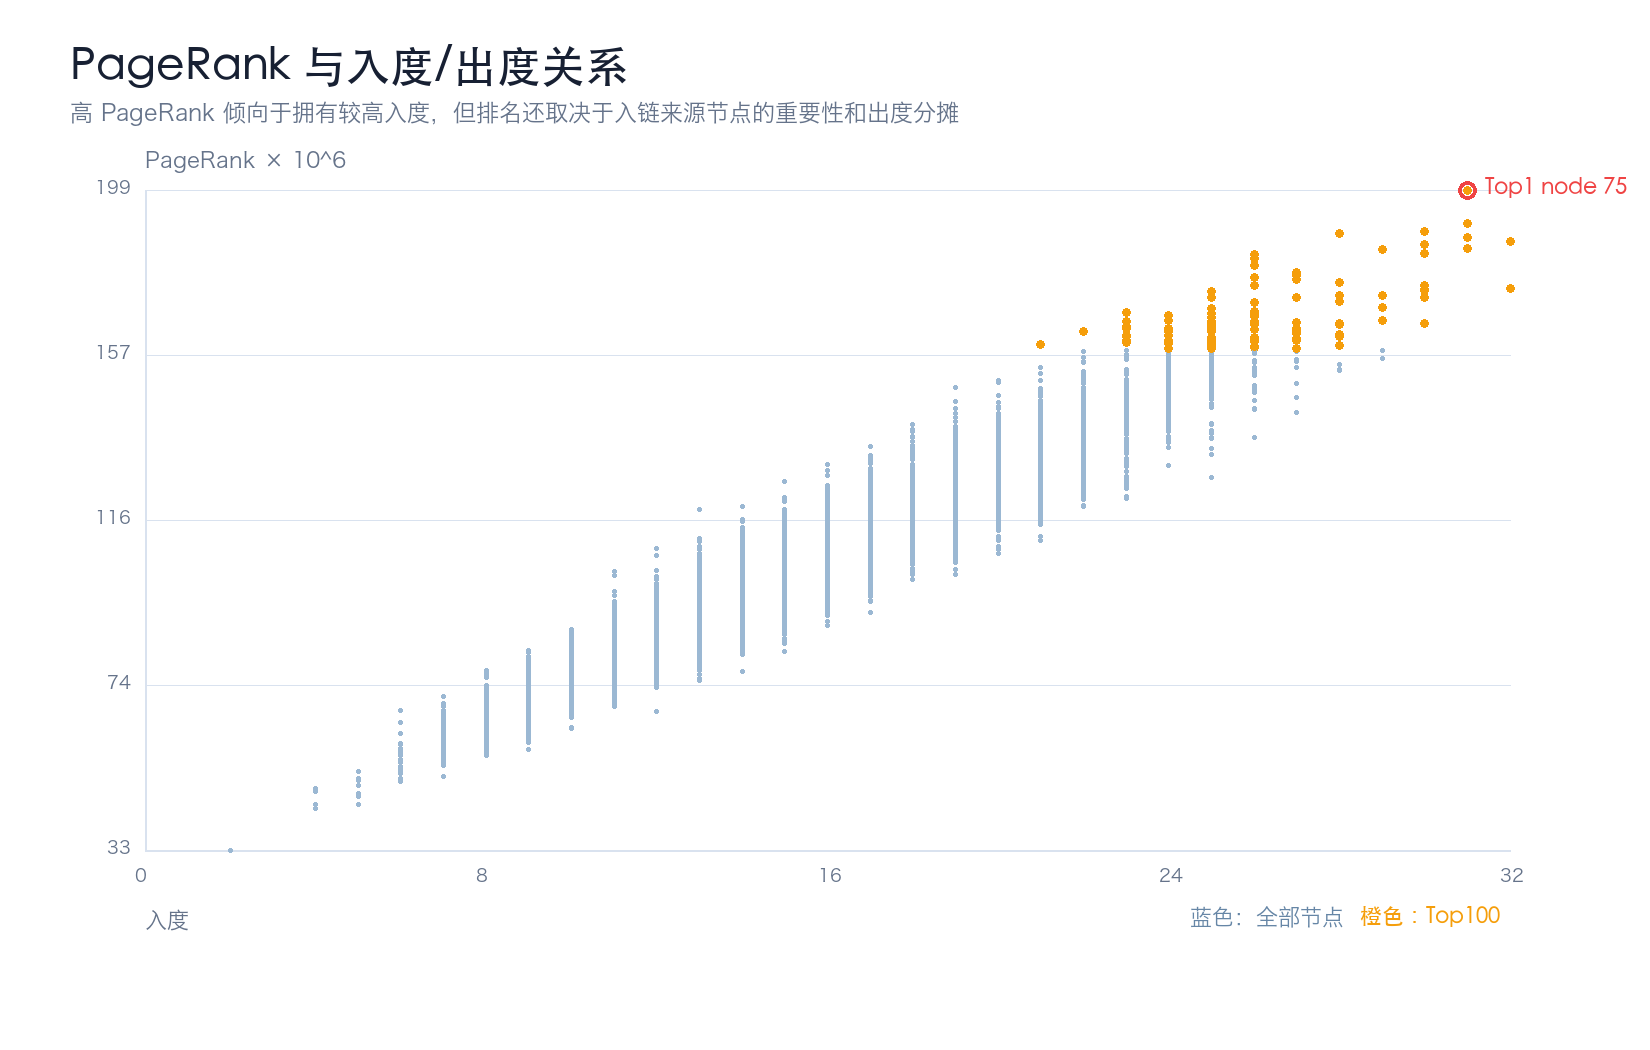
\includegraphics[width=\textwidth]{images/rank_degree_scatter.png}
  \caption{PageRank 分数与入度关系散点图}
  \label{fig:rank-degree}
\end{figure}

\begin{tcolorbox}[colback=green!5!white,colframe=green!50!black,title=性能结果分析]
  \hspace{2em}当前程序的内存主要由节点数组、CSR 图结构、打包边临时数组、索引辅助结构和两个 PageRank 向量构成，空间复杂度为 $O(N+M)$。在 $N=9500$、$M=150000$ 的数据规模下，稠密 double 矩阵理论上约需 688.55 MB，而静态运行峰值 RSS 约 11.23 MB。迭代阶段每轮只线性扫描 dead-end 列表和真实边，17 轮即可达到 $10^{-12}$ 精度，运行时间也明显低于实验要求。
\end{tcolorbox}

\subsection{矩阵规模与内存拆解}

本数据集的邻接矩阵规模为 $9500\times9500=90250000$。实际边数只有 150000，矩阵密度约为 $0.1662\%$，也就是说约 $99.8338\%$ 的矩阵元素为 0。如果用 double 稠密矩阵保存转移概率，矩阵本体需要：

\begin{equation}
9500^2\times8=722000000\ \text{bytes}\approx688.55\ \text{MiB}
\end{equation}

这还不包括 PageRank 向量、输入边、排序临时空间和运行时开销，已经超过实验 80 MB 限制。CSR 只保存真实边和行边界，核心数组空间可按下表估算。

\begin{table}[H]
  \centering
  \caption{主要数据结构内存估算}
  \small
  \begin{tabular}{l c c c}
    \toprule
    \textbf{数据结构} & \textbf{元素数量} & \textbf{单元素字节} & \textbf{估算空间} \\
    \midrule
    \texttt{row\_ptr} & 9501 & 4 & 约 37.1 KB \\
    \texttt{col\_idx} & 150000 & 4 & 约 585.9 KB \\
    \texttt{rank} 与 \texttt{next\_rank} & $2\times9500$ & 8 & 约 148.4 KB \\
    \texttt{node\_ids} & 9500 & 8 & 约 74.2 KB \\
    \texttt{out\_weight} & 9500 & 8 & 约 74.2 KB \\
    \texttt{dead\_nodes} & 1000 & 4 & 约 3.9 KB \\
    dense lookup & 10000 & 4 & 约 39.1 KB \\
    打包边临时数组 & 150000 & 8 & 约 1.14 MB \\
    \bottomrule
  \end{tabular}
\end{table}

核心常驻计算结构低于 1 MB，构图阶段的主要额外开销来自打包边临时数组和节点收集数组。最终静态二进制运行时峰值 RSS 约 11.23 MB，其中包含静态链接运行时、I/O 缓冲、STL 容器容量冗余、栈空间和进程装载开销；即使按进程级峰值统计，也只有限制的约 $14.0\%$。

\subsection{每轮计算量与收敛效率}

PageRank 迭代阶段每轮的主操作是沿 150000 条真实边传播分数。当前 17 轮收敛，因此边传播核心更新次数为：

\begin{equation}
150000\times17=2550000
\end{equation}

除边传播外，每轮还需要一次 dead-end 质量求和、一次 \texttt{next\_rank} 初始化和一次归一化/残差合并遍历。对应复杂度为：

\begin{equation}
O\bigl(T(M+N+|D|)\bigr)
\end{equation}

其中 $T=17$、$M=150000$、$N=9500$、$|D|=1000$。由于 $M$ 远大于 $N$ 和 $|D|$，实际耗时主要由真实边扫描决定。归一化与残差合并后，每轮少一次 $N$ 级向量遍历；出边权重预计算后，每条边传播不再执行除法，只保留一次源节点级乘法和若干目标累加。

\subsection{排名结果的结构解释}

Top-100 节点 PageRank 总和约为 0.01681，Top-20 总和约为 0.00365。Top1 节点 75 的 PageRank 为 0.000198721357091，均匀分布基线为 $1/9500\approx0.000105263157895$，因此 Top1 约为均匀基线的 1.89 倍。Top20 节点 579 的分数仍为 Top1 的约 87.9\%，说明本图不存在极端垄断型中心节点，PageRank 高分区相对平缓。

\begin{table}[H]
  \centering
  \caption{Top 节点与度数关系摘要}
  \small
  \begin{tabular}{c c c c c}
    \toprule
    \textbf{范围} & \textbf{PageRank 质量和} & \textbf{平均入度} & \textbf{平均出度} & \textbf{说明} \\
    \midrule
    全部节点 & 1.00000 & 15.79 & 15.79 & 全图平均水平 \\
    Top-20 & 0.00365 & 28.60 & 18.75 & 入度显著高于平均 \\
    Top-100 & 0.01681 & 26.39 & 16.41 & 高分节点主要集中于高入度区间 \\
    \bottomrule
  \end{tabular}
\end{table}

入度并不等同于 PageRank。节点 75 和 8686 入度同为 31，但节点 75 排名更高，原因是 PageRank 还取决于入链来源节点自身的重要性，以及这些来源节点的出度分摊。节点 725 排名第 5 且出度为 0，说明 dead-end 节点仍可因大量高质量入链获得高分；程序对 dead-end 质量进行回补后，它不会继续向外传播分数，但其当前轮分数会参与全局均分，不会导致概率质量消失。

\subsection{优化收益与取舍}

当前实现没有追求复杂并行或外部库，而是优先选择可解释、可复现、适合提交的优化路径。各优化项的作用边界如下：

\begin{table}[H]
  \centering
  \caption{优化项收益与取舍}
  \small
  \begin{tabularx}{\textwidth}{p{3.2cm} Y Y}
    \toprule
    \textbf{优化项} & \textbf{收益} & \textbf{取舍} \\
    \midrule
    节点压缩 & 数组只按真实节点分配，避免原始 ID 空洞；输出仍能恢复原始编号 & 需要维护 \texttt{node\_ids} 映射表 \\
    dense lookup + fallback & 当前紧凑 ID 上 $O(1)$ 映射；稀疏大 ID 自动回退二分，避免巨大数组 & 代码比单一二分略复杂 \\
    64 位打包边 & 排序去重直接比较整数，减少结构比较开销 & 要通过位运算还原起点和终点 \\
    CSR 稀疏存储 & 空间从 $O(N^2)$ 降到 $O(N+M)$，满足内存限制 & 不直接保存入边，需要按源节点传播 \\
    源节点分块 & 工作集稳定，体现 Block Matrix 思想，便于缓存顺序访问 & 当前数据规模较小，收益主要体现在结构合理性 \\
    权重预计算 & 迭代中避免重复除法 & 多保存一个 \texttt{out\_weight} 数组 \\
    dead-end 列表 & 每轮只扫描 1000 个 dead-end 节点，而不是扫描 9500 个节点判断出度 & 需在构图阶段额外收集列表 \\
    \bottomrule
  \end{tabularx}
\end{table}

因此，本实现的重点不是为了在当前 9500 节点数据上堆叠微优化，而是在满足课程强制要求的同时，让数据表示、数学模型和性能约束保持一致：输入边列表被压缩成 CSR，PageRank 迭代被组织成稀疏矩阵向量乘法，Block Matrix 用源节点块表达，dead-end 和 spider-trap 在公式层面闭合处理。

\section{实验中遇到的问题及解决方法}
\xiaosi

\subsection{原始节点编号不能直接作为数组下标}

如果直接按照原始节点 ID 建立数组，程序会依赖输入编号的连续性。一旦测试数据中节点编号范围很大但实际节点很少，数组会出现大量空洞，甚至造成内存超限。因此最终实现先收集所有出现过的节点，排序去重后使用连续下标计算，并在输出阶段通过 \texttt{node\_ids} 还原原始编号。

\subsection{重复边与 CSR 构建顺序}

边列表输入可能包含重复边。如果在统计出度后才去重，出度和实际参与转移的边数会不一致，导致每条出边分配的概率质量错误。程序先将压缩边打包、排序、去重，再基于去重后的边生成 \texttt{row\_ptr}、\texttt{col\_idx} 和 \texttt{out\_weight}，从根本上保证出度统计与 CSR 中的真实边一致。

\subsection{dead-end 节点会造成概率质量泄漏}

没有出边的节点无法继续向外分配 PageRank。如果忽略这部分节点，每轮迭代都会损失一部分概率质量。程序把所有出度为 0 的节点加入 \texttt{dead\_nodes}，每轮先计算死端节点的总分数，再把这部分质量平均补回所有节点，从而保持 PageRank 向量整体稳定。

\subsection{测试脚本采样间隔可能错过峰值}

作业提供的 \texttt{memoryuse-cpp.py} 每 0.1 秒轮询一次内存，而当前程序单次运行时间也在 0.1 秒量级，轮询脚本可能错过真正峰值。报告中性能结论使用 Linux \texttt{/proc/<pid>/status} 高频读取 \texttt{VmRSS}，并连续运行 5 次取平均，避免单次偶然调度对结论造成影响。

\section{实验结论}
\xiaosi

本实验完成了 PageRank 评分计算程序，并在给定数据集上输出传送参数 $\alpha=0.85$ 时的 Top-100 节点。程序正确处理死端节点和蜘蛛陷阱，最终在 17 轮后收敛，残差约为 $8.064961\times10^{-13}$。

在内存优化方面，程序放弃完整邻接矩阵，采用节点编号压缩、64 位打包边、CSR 稀疏图和源节点行块遍历。迭代阶段结合出边权重预计算、死端节点列表、归一化与残差合并、Top-K 部分排序等优化，使静态 Linux x86-64 可执行文件 5 次运行平均峰值 RSS 约 11.23 MB，远低于 80 MB 限制；平均运行时间约 0.167 秒，也远低于 60 秒限制。

从算法设计看，CSR 稀疏存储将空间复杂度控制为 $O(N+M)$，块遍历把 PageRank 迭代组织为按行块执行的稀疏矩阵向量乘法。最终结果、收敛轮数和性能指标表明，当前实现满足作业对正确性、收敛性、静态编译、稀疏矩阵优化和块矩阵优化的要求。

\section{实验仓库地址}
\xiaosi

本次实验的代码、编译参数、可执行文件与结果文件保存在课程实验仓库中：

\url{https://github.com/IWITRIE/BigDataCourse2026Spring}

\end{document}
